\documentclass[12pt,a4paper]{article}
\usepackage[utf8]{inputenc}
\usepackage[ukrainian]{babel}
\usepackage{amsmath}
\usepackage{amsfonts}
\usepackage{amssymb}
\usepackage{graphicx}
\usepackage{hyperref}
\usepackage[left=2cm,right=2cm,top=2cm,bottom=2cm]{geometry}

% Define custom command for text reference
\newcommand{\textref}[2]{\hyperref[#1]{#2}}
\newcommand{\s}[1]{\texttt{#1}}

\begin{document}

\begin{titlepage}
    \centering
    \vspace*{1cm}

    \Large
    Київський національний університет імені Тараса Шевченка \\

    \vspace{0.5cm}

    \large
    Факультет комп'ютерних наук та кібернетики \\

    \vspace{0.5cm}

    Кафедра інтелектуальних інформаційних систем \\

    \vspace{0.5cm}

    Алгебро-автоматичні методи проектування програмного забезпечення \\

    \vspace{3cm}

    \textbf{Лабораторна робота 6} \\

    \vspace{0.5cm}

    Скінченні автомати \\
    Змоделювати за допомогою часового автомата роботу мікрохвильової пічки.

    \vspace{2cm}

    Виконали студенти 1-го курсу \\

    \vspace{0.2cm}

    Групи ПЗС-1 \\

    \vspace{0.1cm}

    Рябов Кирило \\

    \vspace{0.1cm}

    Соколов Михайло \\

    \vspace{0.1cm}

    Рибачок Руслан \\

    \vfill

    2023

\end{titlepage}

\section*{Лабораторна 6: Змоделювати за допомогою часового автомата роботу мікрохвильової пічки. }

\section{Вступ}

Часові автомати є потужними інструментами в галузі формальної верифікації та моделювання, пропонуючи надійний фреймворк для моделювання та аналізу поведінки систем у реальному часі.

У цьому звіті ми досліджуємо застосування часових автоматів у практичному та повсякденному контексті: моделюванні роботи мікрохвильової печі. Мікрохвильові печі є повсюдними побутовими приладами, які працюють на основі точних часових функцій, що робить їх ідеальним кандидатом для моделювання за допомогою автоматів з часовим інтервалом. Побудувавши та проаналізувавши автомат з годинником, який імітує мікрохвильову піч, ми прагнемо продемонструвати ефективність цих моделей для представлення та перевірки поведінки систем, що працюють у реальному часі.

Структура цього звіту організована наступним чином: Ми починаємо з надання довідкової інформації про часові автомати, представляючи їхні фундаментальні принципи та теоретичні основи. Далі ми моделюємо роботу мікрохвильової печі як автомата з годинником, описуючи його стани, переходи та часові обмеження. Потім ми заглиблюємося в симуляцію та аналіз цієї моделі, за яким слідує перевірка ключових властивостей безпеки. Ми завершуємо доповідь серією тематичних досліджень, які ілюструють реальне застосування нашої моделі, і пропонуємо заключні зауваження щодо ефективності використання автоматів з часовим інтервалом для подібних симуляцій.

\section{Загальні відомості про автомати з годинником}

Часові автомати - це розширення скінченних автоматів, інтегроване з основою для моделювання часу. Вони особливо корисні для аналізу та моделювання систем реального часу, де час настання подій так само важливий, як і послідовність самих подій. Часові автомати дозволяють точно визначати і перевіряти залежну від часу поведінку, що робить їх ідеальними для таких систем, як мікрохвильові печі, де час є критично важливим аспектом функціональності.

\subsection{Визначення часових автоматів}
Автомат з годинником формально визначається як кортеж \( (L, L_0, C, \Sigma, I, E) \) де:
\begin{itemize}
\item \( L \) представляє скінченну множину станів.
\item \( L_0 \subseteq L \) - множина початкових станів.
    \item \( C \) - скінченна множина годинників.
    \item \( \Sigma \) - скінченний алфавіт дій.
    \item \( I: L \rightarrow \text{ClockConstraints}(C) \) визначає значення інваріантів для станів.
\item \( E \subseteq L \times \Sigma \times \text{ClockConstraints}(C) \times 2^C \times L \) - множина ребер, які представляють переходи між станами.
\end{itemize}

\subsection{Принципи та теоретичні основи}
Робота часового автомата базується на двох основних принципах: стани та переходи. Стани в автоматах представляють різні етапи роботи системи, в той час як переходи відображають перехід з одного стану в інший, часто спричинений певними діями або плином часу.

\textbf{Обмеження часу:} Ключовою особливістю часових автоматів є використання годинників, які є змінними, що рівномірно збільшуються з часом. Переходи у часових автоматах можуть бути обумовлені цими змінними за допомогою часових обмежень. Обмеження за часом зазвичай є порівнянням між часом і константою, наприклад, \( x < 5 \) або \( y \geq 3 \).

\textbf{Інтерпретація годинника:} Кожен годинник у часовому автоматі має своє значення, яке зіставляє його з невід'ємним дійсним числом, що представляє проміжок часу. Для множини годинників \( C \), інтерпретація годинника \( \nu \) призначає кожному годиннику \( x \in C \) значення \( \nu(x) \) у \( \mathbb{R}_{\geq 0} \).

\textbf{Переходи та дії за часом:} Часові автомати можуть здійснювати два типи переходів: переходи за часом і переходи за дією. У переходах за часом час просувається у всіх станах, тоді як перехід за дією передбачає зміну стану на основі дії і є миттєвим.

Використовуючи ці принципи, часові автомати можуть імітувати залежну від часу поведінку систем з високою точністю. Це робить їх особливо придатними для моделювання таких систем, як мікрохвильові печі, де час виконання операцій має вирішальне значення для функціональності та безпеки.

\section{Моделювання мікрохвильової печі як часового автомата}

Робота мікрохвильової печі включає в себе кілька ключових станів і переходів, які можна ефективно відобразити за допомогою часового автомата. У цій моделі ми розглядаємо основні функції типової мікрохвильової печі, включаючи запуск, приготування, та зупинку.

\subsection{Опис роботи мікрохвильової печі}
Мікрохвильова піч зазвичай працює в наступних станах:
\begin{itemize}
    \item \textbf{Off:} Стан за замовчуванням, коли піч не використовується.
    \item \textbf{Cooking:} Активний стан, коли піч розігріває їжу.
\end{itemize}

Переходи між цими станами відбуваються внаслідок дій користувача або через певні проміжки часу.

\subsection{Модель автомата з таймером}
Автоматна модель мікрохвильової печі визначається наступним чином:

\vspace{0.5cm}

\textbf{Стани:}
\begin{itemize}
    \item \( S_{\text{off}} \): Вимкнений стан.
    \item \( S_{\text{cooking}} \): Стан приготування.
\end{itemize}

\textbf{Переходи:}
\begin{itemize}
    \item \( S_{\text{off}} \rightarrow S_{\text{cooking}} \): Start cooking.
    \item \( S_{\text{cooking}} \rightarrow S_{\text{off}} \): Stop cooking.
\end{itemize}

\textbf{Часові обмеження:}
\begin{itemize}
    \item Перехід від \( S_{\text{off}} \) до \( S_{\text{cooking}} \) відбувається одразу після дії користувача.
    \item Стан \( S_{\text{cooking}} \) має часове обмеження на основі тривалості приготування, встановленої користувачем.
    \item Перехід до стану \( S_{\text{off}} \) відбувається або після закінчення часу приготування, або коли користувач зупиняє процес приготування.
\end{itemize}

\subsection{Схема автомата і таблиця переходів}
Детальна діаграма автомата та таблиці переходів наведені нижче:

\vspace{0.5cm}

\textbf{Схема автомата:}

\vspace{0.5cm}

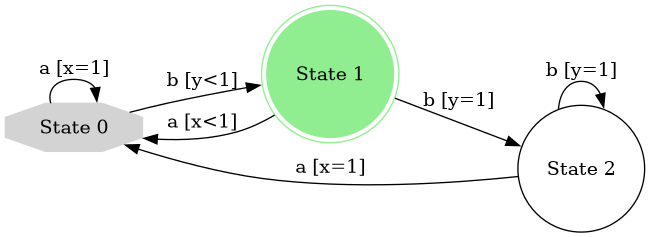
\includegraphics[width=1\textwidth]{timed_automaton.png}

\vspace{0.5cm}

\textbf{Таблиця переходів:} \\

\vspace{0.1cm}

\begin{tabular}{|c|c|c|c|}
\hline
\textbf{From State} & \textbf{To State} & \textbf{Condition/Action} & \textbf{Clock \( x \) Operation} \\
\hline
\( S_{\text{off}} \) & \( S_{\text{cooking}} \) & Start cooking & \( x := 0 \) (Reset clock) \\
\( S_{\text{cooking}} \) & \( S_{\text{off}} \) & Door opened / Stop cooking & \( x := 0 \) (Reset clock) \\
\( S_{\text{cooking}} \) & \( S_{\text{off}} \) & Time elapsed & \( x \geq 120 \) (Stop if 2 mins elapsed) \\
\hline
\end{tabular}

\vspace{0.5cm}

Ця модель відображає основну динаміку роботи мікрохвильової печі, забезпечуючи основу для подальшого моделювання та аналізу з використанням часових автоматів.

\section{Моделювання та аналіз}

У цьому розділі розглядається, як модель часового автомата імітує роботу мікрохвильової печі та аналізується поведінка моделі за різних сценаріїв.

\subsection{Моделювання роботи мікрохвильової печі}
Моделювання роботи мікрохвильової печі з використанням моделі часового автомата передбачає проходження через визначені стани і переходи на основі дій користувача і часових обмежень. Симуляція починається з початкового стану \( S_{\text{off}} \) і рухається через інші стани відповідно до дій користувача і часових обмежень.

\vspace{0.5cm}

\textbf{Алгоритм для моделювання:}
\begin{verbatim}
1. Initialize state to S_off and clock x to 0
2. Loop until simulation ends:
    a. If state == S_off:
       - Wait for user action to start cooking
       - If cooking starts, set state to S_cooking and reset clock x to 0
    b. If state == S_cooking:
       - Increment clock x
       - Check if cooking time has reached 2 minutes (120 seconds)
         If yes, set state to S_off
       - Check for door opened or stop cooking action
         If either occurs, set state to S_off and reset clock x to 0
3. End simulation
\end{verbatim}


Цей алгоритм демонструє прогрес станів у симуляції на основі дій користувача та внутрішнього механізму синхронізації мікрохвильової печі.

\subsection{Аналіз поведінки моделі}
Аналізується поведінка моделі за різних сценаріїв:

\textbf{Стандартна робота:}
У стандартному сценарії роботи мікрохвильова піч переходить зі стану \( S_{\text{off}} \) у стан \( S_{\text{cooking}} \), коли користувач вмикає піч. Вона залишається у режимі \( S_{\text{cooking}} \) до 2 хвилин (120 секунд), а потім автоматично повертається до режиму \( S_{\text{off}} \) після завершення встановленого часу.

\textbf{Втручання користувача:}
У випадку втручання користувача, наприклад, зупинки процесу приготування або відкриття дверцят, модель переходить безпосередньо до \( S_{\text{off}} \), а годинник \( x \) обнуляється. Ця дія означає негайне припинення процесу приготування.

\textbf{Тривалість:}
Якщо задана тривалість готування минає (досягає 2 хвилин), модель переходить від \( S_{\text{cooking}} \) до \( S_{\text{off}} \), що означає кінець циклу готування.

Ці сценарії демонструють, як автоматна модель ефективно імітує роботу мікрохвильової печі, виконуючи стандартні операції, реагуючи на втручання користувача і дотримуючись максимальної тривалості приготування. Це ілюструє здатність моделі відображати як чутливу до часу, так і інтерактивну природу роботи мікрохвильової печі.

\newpage

\section{Перевірка властивостей безпеки}

Перевірка властивостей безпеки в контексті мікрохвильової печі має вирішальне значення для забезпечення безпечної та ефективної роботи приладу. Цей розділ зосереджується на важливості цих властивостей, і методах, які використовуються для їх перевірки у рамках автомата з таймером.

\subsection{Важливість властивостей безпеки}

У мікрохвильовій печі властивості безпеки стосуються забезпечення того, щоб прилад не працював у небезпечних умовах. До основних властивостей належать:

\begin{itemize}
    \item \textbf{Безпека дверцят:} Піч не повинна працювати з відкритими дверцятами.

    \includegraphics[width=1\textwidth]{prop_1.png}

    \vspace{0.5cm}

    \item \textbf{Дотримання часових обмежень:} Час приготування не повинен перевищувати встановлену користувачем тривалість (2 хв).

    \includegraphics[width=1\textwidth]{prop_2.png}
\end{itemize}

\vspace{0.5cm}

Ці властивості є важливими для запобігання нещасним випадкам та забезпечення безпеки користувача.

\subsection{Методи перевірки}
Перевірка цих властивостей у часовому автоматі передбачає аналіз моделі, щоб переконатися, що вона дотримується заданих обмежень і вимог безпеки. Це робиться за допомогою:
\begin{itemize}
    \item \textbf{Перевірка моделі:} Використання автоматизованих інструментів для перевірки дійсності властивостей безпеки у всіх можливих станах.
    \item \textbf{Темпоральна логіка:} Використання формул темпоральної логіки для вираження та перевірки властивостей безпеки у часі.
\end{itemize}

\vspace{0.5cm}

\textbf{Приклад формули часової логіки:}
\begin{verbatim}
G (door_opend -> X (стан = off))
\end{verbatim}
Ця формула, виражена лінійною часовою логікою, стверджує, що якщо дверцята відкриті в будь-який момент (G), то в наступному стані (X) піч повинна бути вимкнена. Це забезпечує властивість безпеки дверцят (детальніше було зображено на двох Рисунках вище).

\vspace{0.5cm}

\textbf{Алгоритм перевірки моделі:}
\begin{verbatim}
1. Define safety properties as temporal logic formulas.
2. For each state in the automaton:
    a. Evaluate the state against all safety formulas.
    b. If any formula is violated, flag the state as unsafe.
3. If all states are safe, the model passes verification.
\end{verbatim}

\section{Приклади та тематичні дослідження}

У цьому розділі наведено реальні приклади та тематичні дослідження, які ілюструють застосування спрощеної моделі автомата з часовим інтервалом, розробленої для мікрохвильової печі. Ці приклади підкреслюють практичність і актуальність моделі для моделювання та аналізу роботи мікрохвильових печей.

\subsection{Приклад 1: Стандартний цикл приготування їжі}
\textbf{Сценарій:} Стандартний цикл приготування, де користувач встановлює час приготування 2 хвилини.

\textbf{Модель застосування:} Часовий автомат переходить від \( S_{\text{off}} \) до \( S_{\text{cooking}} \), дотримуючись часових обмежень. Модель імітує процес приготування протягом заданої тривалості, а потім повертається до \( S_{\text{off}} \) після завершення.

\textbf{Результат:} Модель точно імітує стандартну операцію, демонструючи свою здатність дотримуватися фіксованого часового обмеження у 2 хвилини і автоматично переходити у інший стан після завершення.

\subsection{Приклад 2: Переривання користувача - відчинення дверей}
\textbf{Сценарій:} Користувач відчиняє дверцята мікрохвильової печі під час процесу приготування.

\textbf{Застосування моделі:} Коли дверцята відчиняються, модель переходить з \( S_{\text{cooking}} \) у \( S_{\text{off}} \), а годинник обнуляється, що означає негайну зупинку процесу готування.

\textbf{Результат:} Цей сценарій перевіряє здатність моделі обробляти втручання користувача шляхом негайного переходу до вимкненого стану, що відображає реальну роботу мікрохвильової печі, коли дверцята відчиняються під час приготування їжі.

\subsection{Приклад 3: Автоматичний перехід після закінчення часу}
\textbf{Сценарій:} Забезпечення автоматичного вимкнення мікрохвильової печі після закінчення встановленого часу (2 хвилини).

\textbf{Застосування моделі:} Спостереження за моделлю для забезпечення переходу від \( S_{\text{cooking}} \) до \( S_{\text{off}} \) після досягнення 2-хвилинної позначки, що означає кінець циклу приготування.

\textbf{Результат:} Модель успішно дотримується часового обмеження, автоматично переходячи у вимкнений стан через 2 хвилини, демонструючи свою ефективність у дотриманні заданої тривалості приготування.

\textbf{Висновки:}
Ці приклади демонструють практичне застосування та ефективність моделі часового автомата для моделювання роботи мікрохвильової печі. Вони підкреслюють здатність моделі обробляти операції з фіксованим часом і швидко реагувати на втручання користувача, такі як відкриття дверцят, таким чином підтверджуючи її використання як інструменту для проектування та аналізу систем, чутливих до часу.


\section{Висновки}

У цьому звіті представлено комплексне дослідження використання часового автомата для моделювання роботи мікрохвильової печі. Завдяки структурованій розробці та аналізу моделі ми продемонстрували, як часові автомати можуть ефективно відображати динамічну та чутливу до часу природу функціонування мікрохвильової печі.

\subsection{Підсумок ключових моментів}
\begin{itemize}
    \item Ми визначили і деталізували структуру автоматів з часом, підкресливши їхню придатність для моделювання систем у реальному часі.
    \item Мікрохвильову піч було успішно змодельовано як часовий автомат, з чітко визначеними станами, переходами та часовими обмеженнями.
    \item Моделювання та аналіз показали, що модель точно відображає роботу мікрохвильової печі, включаючи стандартні цикли приготування їжі.
    \item Перевірка властивостей безпеки, були досягнуті, що підкреслює здатність моделі забезпечувати безпеку.
    \item Тематичні дослідження забезпечили реальний контекст, ілюструючи практичне застосування моделі та її ефективність у різних сценаріях.
\end{itemize}

\subsection{Ефективність часових автоматів у моделюванні}
Використання часових автоматів для моделювання мікрохвильової печі виявилося дуже ефективним. Здатність моделі обробляти операції, що базуються на часі, та взаємодію з користувачем, а також забезпечення заходів безпеки, підкреслює переваги часових автоматів у точному представленні складних систем, що працюють у реальному часі.

\subsection{Пропозиції для майбутніх досліджень}
Подальші дослідження можуть розвиватися у кількох напрямках:
\begin{itemize}
    \item \textbf{Складні сценарії:} Включення складніших користувацьких взаємодій та сценаріїв для подальшого тестування надійності моделі.
    \item \textbf{Інтеграція з іншими моделями:} Дослідження інтеграції часових автоматів з іншими обчислювальними моделями для більш комплексного моделювання систем.
    \item \textbf{Автоматизовані засоби верифікації:} Розробка або вдосконалення автоматизованих засобів для ефективнішої перевірки безпеки та експлуатаційних властивостей у часових моделях автоматів.
    \item \textbf{Застосування до інших пристроїв:} Застосування фреймворку часових автоматів до інших побутових або промислових приладів для перевірки його універсальності та ефективності.
\end{itemize}

На завершення, у цьому звіті наведено переконливі аргументи на користь використання часових автоматів у моделюванні та аналізі систем реального часу, особливо в контексті побутових приладів, таких як мікрохвильові печі.

\end{document}
